\documentclass{myclass}
\usepackage[polish]{babel}

% TODO

% * Composite systems made of 2-state systems (2 x 2 & later n x 2 or maybe n x 2 immediately(?))
% * Composite systems: entanglement, density operator, partial trace, no-cloning theorem,
%   decoherence, Bell's theory
%
% * later (after extensively studying composite systems, entanglement, Bell's theory) begin
%   description of quantum registers, gates, idea of computation using those devices (Deutsch,
%   Grover, QFTrans, Shor), applications to number theory, connection with Church-Turing hypothesis.
%   Examples
%
% * possible physical realizations of quantum computing (gates + adiabatic/topological(?)), I'll
%   probably focus on Josephson junctions and charge qubits as they seem most elegant (maybe qdots
%   as well)
%
% * A short overview of classical and quantum information theory (I don't want to go very deep there
%   at the moment): Shannon/Von Neumann entropy, channels, quantum information transfer/cryptography
%   ------
% * General ICT using Ehrenfest theorem
%
%
%

\author{Bartosz Hanc}
% My notes regarding abstract foundations of quantum theory and introduction to quantum computing

\begin{document}

\section{Abstrakcyjna teoria kwantów}

\subsection{Elementy teorii przestrzeni Hilberta}

Przez \(\mathbb{V} := (V,\mathbb{C},+,\cdot)\) będziemy oznaczać przestrzeń wektorową nad ciałem
liczb zespolonych.

\begin{definition}
Odwzorowanie \(d: V \times V \mapsto \mathbb{R}\) będziemy nazywać \textit{metryką} w zbiorze \(V
\neq \emptyset\) iff
\begin{itemize}

\item \(\forall u,v \in V : d(u,v) \geq 0\), przy czym równość zachodzi iff \(u = v\)
(\textit{nieujemność})

\item \(\forall u,v \in V : d(u,v) = d(v,u)\) (\textit{symetria})

\item \(\forall u,v,w \in V : d(u,v) + d(v,w) \geq d(u,w)\) (\textit{nierówność trójkąta})

\end{itemize}
Parę \((V,d(\cdot,\cdot))\) będziemy nazywać \textit{przestrzenią metryczną}.
\end{definition}

\begin{definition}
Niech \((V,d)\) będzie przestrzenią metryczną. Mówimy, iż dany ciąg \((u_n)\) elementów zbioru \(V\)
jest zbieżny do \(g\in V\) tj. \(u_n \to g\) przy \(n \to \infty\) iff \(d(u_n,g) \to 0\) przy \(n
\to \infty\).   
\end{definition}

\begin{definition}
Ciąg \((u_n)\) elementów \(u_n \in V\) będziemy nazywać \textit{ciągiem Cauchy'ego} w przestrzeni
metrycznej \((V,d(\cdot,\cdot))\) iff spełnia on kryterium Cauchy'ego tj.
\begin{equation*}
    \forall \epsilon > 0 : \exists N : \forall n,m > N : d(u_n,u_m) < \epsilon\,.
\end{equation*}  
\end{definition}

\begin{theorem}
Każdy ciąg zbieżny w przestrzeni metrycznej \((V,d)\) jest ciągiem Cauchy'ego w tej przestrzeni.
\end{theorem}

\begin{definition}
Przestrzeń metryczną \((V,d(\cdot,\cdot))\) nazwiemy \textit{zupełną} iff każdy ciąg Cauchy'ego
\((u_n)\) elementów \(u_n \in V\) jest zbieżny do granicy \(g \in V\).
\end{definition}

\begin{definition}
Niech \(\mathbb{V}\) będzie przestrzenią wektorową. Odwzorowanie \(\braket{\cdot} : V \times V
\mapsto \mathbb{C}\) nazwiemy \textit{iloczynem wewnętrznym} wektorów iff
\begin{itemize}
    
    \item \(\forall u,v \in V : \braket{u}{v}^* = \braket{v}{u}\)
    
    \item \(\forall u,v_1,v_2 \in V : \forall \alpha, \beta \in \mathbb{C} : \braket{u}{\alpha v_1 +
    \beta v_2} = \alpha \braket{u}{v_1} + \beta \braket{u}{v_2}\)

    \item \(\forall u \in V : \braket{u} \geq 0\), przy czym równość zachodzi iff \(u =
    \mathsf{0}\). Zauważmy tutaj, iż z pierwszego aksjomatu \(\braket{u} \in \mathbb{R}\), gdyż
    \(\braket{u} = \braket{u}^* \implies \Im{\braket{u}} = 0\). 

\end{itemize}
Parę \((\mathbb{V},\braket{\cdot})\) będziemy nazywać \textit{przestrzenią unitarną}.
\end{definition}

\begin{theorem}
Każda przestrzeń unitarna jest metryczna z metryką indukowaną przez iloczyn wewnętrzny \(d(u,v) :=
\norm{u - v} = \sqrt{\braket{u-v}}\).
\end{theorem}

\begin{theorem}[\textit{Nierówność Cauchy'ego--Schwarza}]
Niech \((\mathbb{V},\braket{\cdot})\) -- przestrzeń unitarna. Wówczas
\begin{equation*}
    \forall u,v \in V : |\braket{u}{v}|^2 \leq \braket{u}\braket{v}\,.
\end{equation*}  
\end{theorem}

\begin{definition}
Przeliczalny zbiór wektorów \(\{v_1,...,v_n\}\) nazwiemy \textit{ortogonalnym} iff 
\begin{equation*}
    \forall i\neq j; i,j\in\{1,...,n\} : \braket{v_i}{v_j} = 0\,.
\end{equation*}
Ten sam zbiór wektorów nazwiemy \textit{ortonormalnym} iff 
\begin{equation*}
    \forall i,j\in\{1,...,n\} : \braket{v_i}{v_j} = \delta_{ij}\,,
\end{equation*}
gdzie \(\delta_{ij}\) jest deltą Kroneckera.
\end{definition}

\begin{theorem}
Każda przestrzeń unitarna \((\mathbb{V}, \braket{\cdot})\) posiada bazę ortonormalną, tj. bazę,
której wektory bazowe tworzą zbiór ortonormalny.
\end{theorem}

\begin{definition}
\textit{Przestrzenią Hilberta} \(\mathscr{H}=(\mathbb{V},\braket{\cdot})\) nazwiemy zupełną
przestrzeń unitarną.
\end{definition}

\begin{definition}
Niech \(\mathscr{H} = (\mathbb{V},\braket{\cdot})\) będzie przestrzenią Hilberta. Odwzorowanie
liniowe \(F:V\mapsto\mathbb{C}\) nazwiemy \textit{funkcjonałem liniowym} w przestrzeni
\(\mathscr{H}\).
\end{definition}

\begin{theorem}
Niech \(V^*\) oznacza zbiór wszystkich funkcjonałów liniowych \(F:V\mapsto\mathbb{C}\). Wówczas
\(\mathbb{V}^*:=(V^*,\mathbb{C},+,\cdot)\), gdzie
\begin{itemize}
    \item \(\forall F_1,F_2 \in V^* : \forall v \in V : (F_1+F_2)(v) = F_1(v) + F_2(v)\)

    \item \(\forall F \in V^* : \forall \alpha \in \mathbb{C} : \forall v \in V : (\alpha \cdot
    F)(v) = \alpha F(v)\)
\end{itemize}
jest przestrzenią wektorową, którą nazywamy \textit{przestrzenią dualną}.
\end{theorem}

\begin{theorem}[\textit{Riesza}]
Niech \(\mathscr{H}=(\mathbb{V},\braket{\cdot})\) będzie przestrzenią Hilberta, a \(\mathbb{V}^*\)
jej przestrzenią dualną. Wówczas istnieje wzajemnie jednoznaczne odwzorowanie wektorów \(v \in V\)
na funkcjonały liniowe \(F \in V^*\). Dodatkowo dla każdego funkcjonału \(F\) istnieje dokładnie
jeden wektor \(u \in V\) taki, że
\begin{equation*}
    \forall v \in V : F(v) = \braket{u}{v}\,.
\end{equation*}
\end{theorem}

\begin{definition}
\textit{Iloczynem Kroneckera} macierzy \(\oper{A} = [a_{ij}]_{n\times m}\) i \(\oper{B} =
[b_{ij}]_{n'\times m'}\) nazywamy macierz wymiaru \(nn'\times mm'\) postaci
\begin{equation*}
    \begin{split}
        \oper{A} \otimes \oper{B} &= \mqty[a_{11} & \cdots & a_{1m} \\ \vdots & \ddots & \vdots \\ a_{n1} & \cdots & a_{nm}] \otimes \mqty[b_{11} & \cdots & b_{1m'} \\ \vdots & \ddots & \vdots \\ b_{n'1} & \cdots & b_{n'm'}] = \mqty[a_{11}\oper{B} & \cdots & a_{1m}\oper{B} \\ \vdots & \ddots & \vdots \\ a_{n1}\oper{B} & \cdots & a_{nm}\oper{B}]
    \end{split}
\end{equation*}
\end{definition}

\begin{definition}
\textit{Iloczynem tensorowym} przestrzeni Hilberta \(\mathscr{H}_1\) i \(\mathscr{H}_2\) o bazach
ortonoromalnych odpowiednio \(\{\phi_i^{(1)}\}\) i \(\{\phi_j^{(2)}\}\) nazywamy przestrzeń Hilberta
\(\mathscr{H} = \mathscr{H}_1 \otimes \mathscr{H}_2\) taką, że:
\begin{itemize}
    
    \item Jej bazą ortonormalną jest zbiór \(\{\phi_i^{(1)} \otimes \phi_j^{(2)}\}\).

    \item Iloczyn wewnętrzny w przestrzeni \(\mathscr{H}_1 \otimes \mathscr{H}_2\) jest zdefiniowany
    jako
    \begin{equation*}
        \braket{\chi_1 \otimes \chi_2}{\psi_1 \otimes \psi_2} := \braket{\chi_1}{\psi_1}_1 \cdot \braket{\chi_2}{\psi_2}_2\,,
    \end{equation*}
    gdzie \(\chi_i,\psi_i \in \mathscr{H}_i\) to pewne wektory, a \(\braket{\cdot}_i\) to iloczyn
    wewnętrzny w \(\mathscr{H}_i\).
\end{itemize}
\end{definition}

\subsection{Notacja Diraca}

Niech \(\mathscr{H}\) będzie przestrzenią Hilberta. Wprowadzimy teraz kompaktową notacją wektorów i
funkcjonałów liniowych wymyśloną przez P.A.M. Diraca. Aby uprościć zapis, będziemy mówili o
wektorach należących do przestrzeni \(\mathscr{H}\) (używając nawet symbolu należenia \(\in
\mathscr{H}\)), mając oczywiście formalnie na myśli wektory należące do zbioru \(V\).

Wektory należące do \(\mathscr{H}\) będziemy oznaczać jako
\begin{equation*}
    \ket{\psi},\, \ket{\phi},\, ...\,,
\end{equation*}
przy czym \(\ket{\cdot}\) to tzw. \textit{ket} i formalnie jest to odwzorowanie \(\ket{\cdot} :
\mathsf{S} \mapsto V\), gdzie \(\mathsf{S}\) jest zbiorem znaków, których używamy do oznaczenia
konkretnych wektorów ze zbioru \(V\). Nie będziemy jednak przestrzegali tego formalnego znaczenia,
utożsamiając dla wygody również  sam symbol z wektorem.

Funkcjonały liniowe należące do przestrzeni dualnej będziemy oznaczać jako
\begin{equation*}
    \bra{\psi},\, \bra{\phi},\, ...\,,
\end{equation*}
przy czym \(\bra{\cdot}\) to tzw. \textit{bra} i formalnie jest to odwzorowanie \(\bra{\cdot} :
\mathsf{S}^* \mapsto V^*\), gdzie \(\mathsf{S}^*\) jest zbiorem znaków, których używamy do
oznaczenia konkretnych funkcjonałów ze zbioru \(V^*\). Ponieważ z tw. Riesza istnieje wzajemnie
jednoznaczne odwzorowanie funkcjonałów liniowych na wektory, więc możemy utożsamić \(\mathsf{S}^* =
\mathsf{S}\).

\subsection{Skończenie wymiarowa przestrzeń Hilberta nad ciałem liczb zespolonych}

Rozważymy teraz konstrukcję skończenie wymiarowej przestrzeni Hilberta złożonej ze skończenie
wymiarowej przestrzeni wektorowej \(\mathbb{V} = (\mathbb{C}^n, \mathbb{C}, +, \cdot)\), której
elementy będziemy w danej bazie \textit{ortonormalnej} \(\{\phi_1, \ldots, \phi_n\}\) zapisywać jako
\begin{equation*}
    \mathbb{V} \ni \ket{\psi} = \sum_{i=1}^n a_i \ket{\phi_i} = \mqty[a_1 \\ \vdots \\ a_n]\,,
\end{equation*}
gdzie \(a_i = \braket{\phi_i}{\psi}\in\mathbb{C}\) oraz iloczynu wewnętrznego zdefiniowanego jako
\begin{equation*}
    \braket{ \sum_{i=1}^n a_i \ket{\phi_i}}{ \sum_{i=1}^n b_i \ket{\phi_i}} := \sum_{i=1}^n a_{i}^*b_i\,.
\end{equation*}
Powstała w ten sposób skończenie wymiarowa przestrzeń unitarna jest trywialnie zupełna, a zatem
skonstruowaliśmy skończenie wymiarową przestrzeń Hilberta. Wektor w tej przestrzeni możemy utożsamić
(poprzez iloczyn wewnętrzny) z macierzą kolumnową jego współrzędnych w danej bazie ortonormalnej.
Jasne jest również czym jest funkcjonał liniowy stowarzyszony z danym wektorem
\begin{equation*}
    \bra{\psi} = \mqty[a_1 \\ \vdots \\ a_n]^\dagger = \mqty[a_1^* & \ldots & a_n^*]\,,
\end{equation*}
gdzie \(\dagger\) oznacza \textit{sprzężenie hermitowskie} macierzy, tj. sprzężoną macierz
transponowaną. W dalszej części skupimy się głównie na skończenie wymiarowych przestrzeniach
Hilberta \(((\mathbb{C}^n, \mathbb{C}, +, \cdot),\braket{\cdot})\), gdyż stanowią one podstawę opisu
teorii obliczeń kwantowych i kwantowej teorii informacji. Należy zdawać sobie jednak sprawę, iż
stanowi to duże uproszczenie w stosunku do wymagań pełnoprawnych teorii fizycznych (mechanika
falowa, kwantowa teoria pola), w których niezbędna jest teoria nieskończenie wymiarowych przestrzeni
Hilberta.

\subsection{Elementy teorii operatorów liniowych}

\begin{definition}
\textit{Operatorem liniowym} \(\oper{A}\) w przestrzeni \(\mathscr{H} = (\mathbb{V},
\braket{\cdot})\) nazywamy odwzorowanie liniowe 
\begin{equation*}
    \oper{A} : D(\oper{A}) \mapsto D(\oper{A})\,,
\end{equation*}
gdzie \(D(\oper{A})\) jest pewną podprzestrzenią wektorową przestrzeni \(\mathbb{V}\). Dodatkowo
zakładamy, iż dziedziny operatorów są gęste, to znaczy ich domknięcia są równe \(\mathscr{H}\).
\end{definition}

Zgodnie z wcześniejszymi komentarzami nie będziemy wnikali w subtelne problemy wynikające z faktu,
iż w nieskończenie wymiarowej przestrzeni Hilberta pojęcie operatora liniowego jest nieodłącznie
związane z pojęciem dziedziny tego operatora, który w ogólności nie jest określony na całej
przestrzeni Hilberta, a tylko na pewnym jej podzbiorze. Komplikacje te nie występują w skończenie
wymiarowych przestrzeniach Hilberta wymiaru \(n\), w których operatory liniowe możemy utożsamiać z
\textit{endomorfizmami} tej przestrzeni
\begin{equation*}
\oper{A}: V \mapsto V\,.
\end{equation*}

Jak wiadomo z elementarnej algebry w przypadku \(n\)--wymiarowej przestrzeni wektorowej każdemu
endomorfizmowi \(\oper{A}\) możemy przyporządkować macierz wymiaru \(n\times n\), której elementy w
danej bazie ortonormalnej \(\{\phi_1,\ldots,\phi_n\}\) są dane przez wartości \(\oper{A}\) na
wektorach bazowych
\begin{equation*}
\begin{split}
\oper{A}\ket{\phi_1} &= A_{11}\ket{\phi_1} + A_{21}\ket{\phi_2} + \ldots + A_{n1}\ket{\phi_n}\\
&\vdots\\
\oper{A}\ket{\phi_n} &= A_{1n}\ket{\phi_1} + A_{2n}\ket{\phi_2} + \ldots + A_{nn}\ket{\phi_n}
\end{split}\quad,
\end{equation*}
skąd element \(A_{ij}\) macierzy \(\oper{A}\) w bazie ortonormalnej \(\{\phi_i\}\) jest dany przez
\begin{equation*}
A_{ij} = \bra{\phi_i}\oper{A}\ket{\phi_j}\,.
\end{equation*}

\begin{definition}
\textit{Sprzężeniem} operatora \(\oper{A}\) nazywamy operator \(\oper{A}^\dagger\) zdefiniowany
(pomijając wszelkie problemy związane z określeniem dziedzin operatorów) przez równanie
\begin{equation*}
\forall \psi,\phi\in\mathscr{H}: \bra{\psi}\oper{A}^\dagger\ket{\phi} = \bra{\phi}\oper{A}\ket{\psi}^*\,.
\end{equation*}
\end{definition}

Podstawiając w miejsce wektorów \(\psi\), \(\phi\) wektory bazy otrzymujemy (w przypadku skończenie
wymiarowych przestrzeni Hilberta) zależność między macierzą \(\oper{A}\) i jej sprzężeniem
hermitowskim \(\oper{A}^\dagger\)
\begin{equation*}
A^\dagger_{ij} = A_{ji}^*\,.
\end{equation*} 

\begin{definition}
\textit{Komutatorem} operatorów \(\oper{A}\), \(\oper{B}\) operator \([\oper{A},\oper{B}]\)
zdefiniowany jako
\begin{equation*}
\forall \psi \in D : [\oper{A},\oper{B}]\psi = \oper{A}\oper{B}\psi - \oper{B}\oper{A}\psi\,. 
\end{equation*}
Jeśli \([\oper{A},\oper{B}] = \oper{\mathsf{0}}\) (gdzie \(\oper{\mathsf{0}}\) oznacza
\textit{operator zerowy} \(\oper{\mathsf{0}}\psi=\mathsf{0}\)), to mówimy, że operatory
\(\oper{A}\), \(\oper{B}\) \textit{komutują}.
\end{definition}

\begin{definition}
\textit{Antykomutatorem} operatorów \(\oper{A}\), \(\oper{B}\) nazywamy operator
\(\{\oper{A},\oper{B}\}\) zdefiniowany jako
\begin{equation*}
    \{\oper{A},\oper{B}\}\psi := \oper{A}\oper{B}\psi + \oper{B}\oper{A}\psi\,.
\end{equation*}
\end{definition}

\begin{theorem}
Dla dowolnych operatorów \(\oper{A}\), \(\oper{B}\), \(\oper{C}\) zakładając odpowiednie dziedziny,
zachodzi:
\begin{itemize}
    \item \([\oper{A} + \oper{B},\oper{C}] = [\oper{A},\oper{C}] + [\oper{B},\oper{C}]\) ;
    \item \([\oper{A}\oper{B},\oper{C}] = \oper{A}[\oper{B},\oper{C}] +
    [\oper{A},\oper{C}]\oper{B}\) .
    \item \([[\oper{A}, \oper{B}], \oper{C}] + [[\oper{B},\oper{C}],\oper{A}] + [[\oper{C},
    \oper{A}], \oper{B}] = \oper{0}\) (\textit{tożsamość Jacobiego})
\end{itemize}   
\end{theorem}

\begin{definition}
\textit{Ślad operatora \(\oper{A}\)} definiujemy jako liczbę \(\Trace \oper{A} \in \mathbb{C}\)
równą
\begin{equation*}
\Trace{\oper{A}} := \sum_{i} \bra{\phi_i}\oper{A}\ket{\phi_i}\,,
\end{equation*}
gdzie \(\{\phi_i\}\) jest dowolną ortonormalną bazą przestrzeni \(\mathscr{H}\).
\end{definition}

\begin{theorem}
Ślad operatora nie zależy od wyboru ortonormalnej bazy przestrzeni Hilberta.    
\end{theorem}

\begin{theorem} Podstawowe własności śladu.
\begin{itemize}
    \item Operacja wzięcia śladu operatora jest liniowa tj. 
    \begin{equation*}
        \Trace(\alpha\oper{A} + \beta\oper{B}) = \alpha\Trace(\oper{A}) + \beta\Trace(\oper{B})\,.
    \end{equation*}

    \item Dla dowolnych operatorów \(\oper{A}\), \(\oper{B}\), \(\oper{C}\) zachodzi
    \begin{equation*}
        \Trace{\oper{ABC}} = \Trace{\oper{BCA}} = \Trace{\oper{CAB}}\,.
    \end{equation*}

    \item \(\Trace{\oper{A}} = \left(\Trace{\oper{A}^\dagger}\right)^*\)
    \item \(\det{\e^{\oper{A}}} = \e^{\Trace{\oper{A}}}\)
\end{itemize}  
\end{theorem}

\begin{definition}[\textit{Funkcja operatora}]
Niech \(f(x):\mathbb{R}\mapsto\mathbb{R}\) będzie funkcją zmiennej rzeczywistej taką, że istnieje
szereg potęgowy
\begin{equation*}
\sum_{n=0}^\infty\frac{a_n}{n!}x^n\,,
\end{equation*}
który jest zbieżny jednostajnie na \(\mathbb{R}\) do \(f\). Wówczas funkcję operatora
\(f(\oper{A})\) definiujemy jako
\begin{equation*}
f(\oper{A}) := \sum_{n=0}^\infty \frac{a_n}{n!}\oper{A}^n\,,
\end{equation*}
gdzie przyjmujemy \(\oper{A}^0 := \oper{I}\). W szczególności mamy
\begin{itemize}
    \item \(\exp(\oper{A}) := \sum_{n=0}^\infty \frac{1}{n!}\oper{A}^n\)

    \item \(\sin(\oper{A}) := \sum_{n=0}^\infty \frac{(-1)^n}{(2n+1)!}\oper{A}^{2n+1}\)

    \item \(\cos(\oper{A}) := \sum_{n=0}^\infty \frac{(-1)^n}{(2n)!}\oper{A}^{2n}\)
\end{itemize}
\end{definition}

W teorii kwantowej główną rolę odgrywają trzy rodziny operatorów: operatory samosprzężone, rzutowe i
unitarne.

\linesep

\begin{definition}
    \textit{Operatorem samosprzężonym} (pomijając wszelkie problemy związane z określeniem dziedzin
    operatorów) nazywamy operator \(\oper{A}\), dla którego \(\oper{A} = \oper{A}^\dagger\).
\end{definition}

W przypadku skończenie wymiarowych przestrzeni Hilberta definicja ta jest pełna, a operatory
samosprzężony możemy utożsamiać z macierzami hermitowskimi tj. macierzami, których elementy
spełniają związek
\begin{equation*}
    A_{ij} = A_{ji}^*\,.
\end{equation*}

W przypadku nieskończenie wymiarowych przestrzeni Hilberta definicja ta jest niepełna gdyż trzeba
mieć świadomość, iż równość operatorów oznacza z definicji równość ich dziedzin, co wymaga
wprowadzenia rozróżnienia między operatorami jedynie \textit{symetrycznymi} (tj. spełniającymi
równość \(\bra{\psi}\oper{A}\ket{\phi} = \bra{\phi}\oper{A}\ket{\psi}^*\) dla dowolnych
\(\psi,\phi\in D(\oper{A})\)), a operatorami samosprzężonymi.

Operatory samosprzężone odgrywają wyróżnioną rolę w teorii kwantowej ze względu na trzy twierdzenia,
które są dla nich spełnione.

\begin{theorem}
Wartości własne operatora samosprzężonego są liczbami rzeczywistymi.   
\end{theorem}

\begin{theorem}
Zbiór wektorów własnych operatora samosprzężonego rozpina przestrzeń \(\mathscr{H}\).   
\end{theorem}

\begin{theorem}
Jeśli widmo operatora samosprzężonego nie jest zdegenerowane, to wektory własne tworzą zbiór
ortogonalny.
\end{theorem}

\linesep

\begin{definition}
\textit{Operatorem rzutowym} nazywamy operator \(\oper{P}\) taki, że \(\oper{P} = \oper{P}^\dagger\)
(samosprzężoność) i \(\oper{P}^2 = \oper{P}\) (idempotentność). 
\end{definition}

Ważnym przykładem operatora rzutowego jest operator rzutowania na jednowymiarową podprzestrzeń
rozpiętą na unormowanym wektorze \(\ket{\phi}\) (rzutowanie na kierunek wektora \(\phi\)), który w
notacji Diraca możemy zapisać jako \(\oper{P} = \ket{\phi}\bra{\phi}\) tj. \(\forall \psi :
\oper{P}(\psi) = \braket{\phi}{\psi}\phi\). Jest to oczywiście operator liniowy, gdyż dla dowolnych
wektorów \(\ket{\psi_1}\), \(\ket{\psi_2}\) i skalarów \(\alpha\), \(\beta\) mamy
\begin{equation*}
    \begin{split}
        &\ket{\phi}\bra{\phi}(\alpha\ket{\psi_1} + \beta\ket{\psi_2}) = \ket{\phi}\braket{\phi}{\alpha\psi_1 + \beta\psi_2} \\
        &= \alpha\ket{\phi} \braket{\phi}{\psi_1} + \beta\ket{\phi}\braket{\phi}{\psi_2}\,.
    \end{split}
\end{equation*}
Jest również idempotentny, gdyż 
\begin{equation*}
    \ket{\phi}\bra{\phi}(\ket{\phi}\braket{\phi}{\psi}) =  \ket{\phi}\braket{\phi}{\psi}
\end{equation*}
z założenia \(\braket{\phi} = 1\) oraz samosprzężony
\begin{equation*}
    (\braket{\psi_1}{\phi}\braket{\phi}{\psi_2})^* = \braket{\psi_1}{\phi}^*\braket{\phi}{\psi_2}^* = \braket{\phi}{\psi_1}\braket{\psi_2}{\phi} = \braket{\psi_2}{\phi}\braket{\phi}{\psi_1}\,.
\end{equation*}
Łatwo pokazać również, iż jeśli \(\{\phi_i\}\) jest ortonormalnym zbiorem wektorów, to
\begin{equation*}
    \oper{P} = \sum_i \ket{\phi_i}\bra{\phi_i}
\end{equation*}
jest operatorem rzutowym. W szczególności, jeśli \(\{\phi_i\}\) jest ortonormalną bazą przestrzeni
\(\mathscr{H}\), to
\begin{equation*}
    \sum_i \ket{\phi_i}\bra{\phi_i} = \oper{I}\,.
\end{equation*}

\linesep

\begin{definition}
\textit{Operatorem unitarnym} nazywamy operator \(\oper{U}\) taki, że
\begin{equation*}
    \oper{U}\oper{U}^\dagger = \oper{U}^\dagger\oper{U} = \oper{I}\,.
\end{equation*}
\end{definition}

Przekształcenia unitarne reprezentowane przez operatory unitarne mają użyteczną własność polegającą
na zachowywaniu wartości iloczynu wewnętrznego dwóch wektorów, a zatem w szczególności normy wektora
\begin{equation*}
    \braket{\oper{U}\psi}{\oper{U}\phi} = \braket{\oper{U}^\dagger\oper{U}\psi}{\phi} = \braket{\psi}{\phi}\,.
\end{equation*}

\linesep

\begin{textbox}
\begin{theorem}[\textit{spektralne}]
Niech \(\mathscr{H}\) będzie przestrzenią Hilberta. Dla każdego samosprzężonego operatora liniowego
\(\oper{A}\) w \(\mathscr{H}\) istnieje unikalna rodzina operatorów rzutowych \(\oper{P}(\lambda)\)
indeksowanych ciągłym parametrem \(\lambda \in \mathbb{R}\) taka, że
\begin{itemize}
    
    \item \(\oper{P}(\lambda_1)\oper{P}(\lambda_2) = \oper{P}(\min(\lambda_1,\lambda_2))\)

    \item \(\forall \lambda: \lim_{\epsilon\to0^+}\oper{P}(\lambda+\epsilon) = \oper{P}(\lambda)\)
    
    \item \(\lim_{\lambda\to-\infty}\oper{P}(\lambda) = \oper{0}\)

    \item \(\lim_{\lambda\to+\infty}\oper{P}(\lambda) = \oper{I}\)

    \item \(\oper{A} = \int\limits_{-\infty}^{+\infty}\lambda \dd{\oper{P}(\lambda)}\)

\end{itemize}
gdzie ostatnia całka to tzw. \textit{całka Riemanna--Stieltjesa} względem miary operatorowej
zdefiniowana jako
\begin{equation*}
        \int\limits_a^b f(x) \dd{\sigma(x)} := \lim_{n\to\infty}\sum_{k=1}^nf(x_k)\left[\sigma(x_k) - \sigma(x_{k-1})\right]\,,
\end{equation*}
dla 
\begin{equation*}
    f: \mathbb{R} \mapsto \mathbb{R}\,,\quad \sigma: \mathbb{R} \mapsto X\,,
\end{equation*}
gdzie \([a;b] = \bigcup_{k=1}^{n}[x_{k-1}; x_k]\) jest podziałem normalnym odcinka \([a;b]\).
Dodatkowo dla dowolnej funkcji operatora \(f\) zachodzi
\begin{equation*}
    f(\oper{A}) = \int\limits_{-\infty}^{+\infty} f(\lambda) \dd{\oper{P}(\lambda)}\,.
\end{equation*}
\end{theorem}        
\end{textbox}

W szczególnym przypadku, gdy operator samosprzężony \(\oper{A}\) ma niezdegenerowane widmo
\(\{\lambda_i\}\) będące zbiorem przeliczalnym, wiemy, że zbiór unormowanych wektorów własnych
\(\{\phi_i\}\) jest bazą ortonormalną przestrzeni \(\mathscr{H}\), czyli dla dowolnego wektora
\(\psi \in \mathscr{H}\) możemy zapisać
\begin{equation*}
    \ket{\psi} = \sum_{i} c_i\ket{\phi_i} = \sum_{i} \braket{\phi_i}{\psi}\ket{\phi_i}\,,
\end{equation*}
gdzie \(c_i = \braket{\phi_i}{\psi} \in \mathbb{C}\) to współrzędne wektora w zadanej bazie.
Działając operatorem \(\oper{A}\) na wektor \(\psi\) mamy
\begin{equation*}
    \oper{A}\ket{\psi} = \sum_{i} \braket{\phi_i}{\psi}\oper{A}\ket{\phi_i} =
    \sum_{i} \braket{\phi_i}{\psi}\lambda_i\ket{\phi_i} = \left(\sum_i\lambda_i\ket{\phi_i}\bra{\phi_i}\right)\ket{\psi} \,.
\end{equation*}
Całka Stieltjesa z twierdzenia spektralnego przechodzi więc w tym przypadku w sumę (być może
nieskończoną) operatorów rzutowych rzutujących na jednowymiarowe podprzestrzenie rozpięte na
kolejnych wektorach własnych operatora
\begin{equation*}
    \oper{A} = \sum_{i} \lambda_i \ket{\phi_i}\bra{\phi_i}\,.
\end{equation*}

\subsection{Postulaty teorii kwantów}

Poniżej przedstawiono postulaty ogólnej, abstrakcyjnej teorii kwantów. Postulaty te obowiązują we
wszystkich realizacjach teorii kwantów np. mechanice falowej, czy kwantowej teorii pola, jednak ze
względu na swój ogólny charakter same w sobie nie dostarczają narzędzi do rozwiązywania żadnych
konkretnych problemów fizycznych. Nie należy ich również traktować jako podstaw do aksjomatyzacji
teorii kwantowej. Stanowią one raczej sposób uporządkowania w spójną strukturę wiedzy dotyczącej
konkretnych realizacji teorii kwantów
\medskip

\begin{enumerate}[label=\Roman*.]
    
    \item \textbf{O modelu matematycznym.} Modelem matematycznym teorii kwantów jest teoria
    przestrzeni Hilberta nad ciałem liczb zespolonych i teoria operatorów liniowych działających w
    tej przestrzeni.

    \item \textbf{O pytaniach elementarnych.} Pytaniem elementarnym nazwiemy pytanie, na które
    odpowiedź może brzmieć jedynie ,,TAK'' lub ,,NIE''. Pytanie elementarne nazwiemy rozstrzygalnym
    w obrębie danej teorii kwantowej iff istnieje wzajemnie jednoznaczne przyporządkowanie tego
    pytania do pewnego operatora rzutowego \(\oper{P}\). Będziemy wówczas mówili, iż dane pytanie
    elementarne jest reprezentowane przez \(\oper{P}\). Każde pytanie elementarne reprezentowane
    przez \(\oper{P}\) można zanegować otrzymując pytanie reprezentowane przez \(\oper{I} -
    \oper{P}\) (zauważmy, że \((\oper{I} - \oper{P})^2 = \oper{I} - \oper{P}\)), natomiast dwa
    pytania elementarne reprezentowane przez \(\oper{P}_1\) i \(\oper{P}_2\) można połączyć
    spójnikiem
    \begin{itemize}
        \item ,,I''; otrzymując pytanie reprezentowane przez \(\oper{P}_1\oper{P}_2\), przy czym z
        oczywistych względów musi zachodzić \([\oper{P}_1, \oper{P}_2] = \oper{\mathsf{0}}\)

        \item ,,LUB''; otrzymując pytanie reprezentowane przez \(\oper{P}_1 + \oper{P}_2\), przy
        czym musi zachodzić \(\oper{P}_1\oper{P}_2 = \oper{\mathsf{0}}\) (istotnie \((\oper{P}_1 +
        \oper{P}_2)^2 = \oper{P}_1 + \oper{P}_2 \)).

    \end{itemize}

    \item \textbf{O stanach układu.} Stan prostego układu fizycznego jest reprezentowany przez
    unormowany wektor \(\ket{\Psi}\) w abstrakcyjnej przestrzeni Hilberta \(\mathscr{H} =
    (\mathbb{V}, \braket{\cdot})\), przy czym utożsamiamy ze sobą wektory różniące się jedynie
    globalnym czynnikiem fazowym tj. \(\ket{\Psi} \cong \e^{\im\alpha}\ket{\Psi}\) dla \(\alpha \in
    \mathbb{R}\).

    \item \textbf{O prawdopodobieństwach.} Teoria kwantowa dostarcza jedynie probabilistycznych
    odpowiedzi na rozstrzygalne pytania elementarne. Prawdopodobieństwo \(p\), iż odpowiedź na
    pytanie elementarne reprezentowane przez \(\oper{P}\) jest twierdząca, dla układu
    reprezentowanego przez \(\Psi\) wynosi
    \begin{equation*}
        p = \bra{\Psi}\oper{P}\ket{\Psi}\,.
    \end{equation*}
    Zauważmy, iż trywialnie \(p\in\mathbb{R}\) oraz z nierówności Cauchy'ego--Schwarza mamy
    \begin{equation*}
        p^2 \leq \braket{\Psi} \braket{\oper{P}\Psi} = \bra{\Psi}\oper{P}^2\ket{\Psi} = p\,,
    \end{equation*}
    skąd \(p(p-1) \leq 0\), czyli \(p \in [0;1]\).

    \item \textbf{O wielkościach fizycznych.} Każda wielkość fizyczna \(A\) występująca w danej
    teorii kwantowej jest reprezentowana przez samosprzężony operator liniowy \(\oper{A}\) i
    stowarzyszoną z nim na mocy twierdzenia spektralnego rodzinę operatorów rzutowych
    \(\oper{P}_A(\lambda)\). Operator rzutowy \(\oper{P}_A(\lambda)\) reprezentuje pytanie:
    \textit{czy wielkość fizyczna \(A\) ma wartość nie większą od \(\lambda\)?}, natomiast operator
    rzutowy \(\oper{I}-\oper{P}_A(\lambda)\): \textit{czy wielkość fizyczna \(A\) ma wartość większą
    od \(\lambda\)?} Na mocy postulatu drugiego możemy skonstruować pytanie: \textit{czy wielkość
    fizyczna \(A\) ma wartość z przedziału \((\lambda_1;\lambda_2]\)?}, reprezentowane przez
    operator 
    \begin{equation*}
        (\oper{I} - \oper{P}_A(\lambda_1))\oper{P}_A(\lambda_2) =
        \oper{P}_A(\lambda_2)-\oper{P}_A(\lambda_1)\,.
    \end{equation*}
    Wartość oczekiwaną wielkości \(A\) dla układu reprezentowanego przez \(\Psi\) obliczamy jako
    \begin{equation*}
        \langle A \rangle = \bra{\Psi}\oper{A}\ket{\Psi}\,.
    \end{equation*}

    \item \textbf{O ewolucji układu w czasie.} Prawdopodobieństwo \(p\) odpowiedzi twierdzącej na
    pytanie \(\oper{P}\) dla układu reprezentowanego przez \(\Psi\) ewoluuje w czasie zgodnie z
    \begin{equation*}
        p(t) = \bra{\Psi(t)}\oper{P}\ket{\Psi(t)}\,,
    \end{equation*}
    gdzie wektory stanu \(\ket{\Psi}\) ewoluują zgodnie z \textit{równaniem Schr\"{o}dingera}
    \begin{equation*}
        \oper{H}\ket{\Psi} = \im\hbar\partial_t\ket{\Psi}\,,
    \end{equation*}
    gdzie \(\oper{H}(t)\) jest specjalnym operatorem samosprzężonym (zwanym operatorem Hamiltona lub
    po prostu hamiltonianem) reprezentującym hamiltonian układu, tworzonym wedle określonych reguł w
    danej realizacji teorii kwantów, natomiast \(\hbar\) to stała fizyczna o wymiarze działania
    \begin{equation*}
        \hbar = \frac{h}{2\pi} = 1.054571817\ldots \cdot 10^{-34}\,\text{J}\cdot\text{s}
    \end{equation*}
    zwana \textit{zredukowaną stałą Plancka}.
    
    \item \textbf{O układach złożonych.} Przestrzeń Hilberta \(\mathscr{H}\) układu złożonego ma
    strukturę iloczynu tensorowego przestrzeni Hilberta układów prostych wchodzących w jego skład
    \(\mathscr{H}=\mathscr{H}_1\otimes\mathscr{H}_2\otimes\ldots\otimes\mathscr{H}_n\) .

\end{enumerate}

\subsection{Zasada nieoznaczoności}

Niech \(A\) będzie pewną wielkością fizyczną reprezentowaną przez operator \(\oper{A}\). Zdefiniujmy
odchylenie standardowe \(\sigma_A \geq 0\) wielkości \(A\) dla układu w stanie \(\Psi\) jako
\begin{equation*}
    \sigma_A^2 := \langle (A - \langle A \rangle)^2 \rangle = \braket{(\oper{A}-a)\Psi}{(\oper{A}-a)\Psi}\,,
\end{equation*}
gdzie \(a = \expval{A}\) jest wartością oczekiwaną wielkości \(A\). Dla dowolnych dwóch wielkość
fizycznych \(A\) i \(B\) w układzie reprezentowanym przez \(\Psi\) mamy z nierówności
Cauchy'ego--Schwarza
\begin{equation*}
    \sigma_A^2\sigma_B^2 \geq \left|\braket{(\oper{A}-a)\Psi}{(\oper{B}-b)\Psi}\right|^2\,.
\end{equation*}
Jednocześnie dla dowolnego \(z = x + \im y \in\mathbb{C}\) mamy
\begin{equation*}
    |z|^2 = x^2 + y^2 = \left(\frac{z + z^*}{2}\right)^2 + \left(\frac{z-z^*}{2\im}\right)^2\,.
\end{equation*}
Z powyższego mamy więc
\begin{equation*}
    \sigma_A^2\sigma_B^2 \geq \left[\frac{1}{2\im}\left(\braket{\oper{\mathcal{A}}\Psi}{\oper{\mathcal{B}}\Psi} - \braket{\oper{\mathcal{B}}\Psi}{\oper{\mathcal{A}}\Psi}\right)\right]^2 + \left[\frac{1}{2}(\braket{\oper{\mathcal{A}}\Psi}{\oper{\mathcal{B}}\Psi} + \braket{\oper{\mathcal{B}}\Psi}{\oper{\mathcal{A}}\Psi})\right]^2\,,
\end{equation*}
gdzie \(\oper{\mathcal{A}} := \oper{A} - a\), \(\oper{\mathcal{B}} := \oper{B} - b\). Jednocześnie
\begin{equation*}
    \begin{split}
        &\braket{\oper{\mathcal{A}}\Psi}{\oper{\mathcal{B}}\Psi} - \braket{\oper{\mathcal{B}}\Psi}{\oper{\mathcal{A}}\Psi} =
        \bra{\Psi}(\oper{\mathcal{A}}\oper{\mathcal{B}}\ket{\Psi}-\oper{\mathcal{B}}\oper{\mathcal{A}}\ket{\Psi})=\\
        &\bra{\Psi}[\oper{\mathcal{A}},\oper{\mathcal{B}}]\ket{\Psi} = \bra{\Psi}[\oper{A},\oper{B}]\ket{\Psi}\,.
    \end{split}
\end{equation*}
oraz
\begin{equation*}
    \braket{\oper{\mathcal{A}}\Psi}{\oper{\mathcal{B}}\Psi} + \braket{\oper{\mathcal{B}}\Psi}{\oper{\mathcal{A}}\Psi} = \bra{\Psi}\{\oper{\mathcal{A}},\oper{\mathcal{B}}\}\ket{\Psi} = \bra{\Psi}\{\oper{A},\oper{B}\}\ket{\Psi} - 2\expval{A}\expval{B}
\end{equation*}
Ostatecznie otrzymujemy więc
\begin{equation*}
    \boxed{
    \sigma_A^2\sigma_B^2 \geq \left(\frac{1}{2\im}\bra{\Psi}[\oper{A},\oper{B}]\ket{\Psi}\right)^2 + \left(\frac{1}{2}\bra{\Psi}\{\oper{A},\oper{B}\}\ket{\Psi} - \expval{A}\expval{B}\right)^2
    }\quad.
\end{equation*}
Powyższą nierówność nazywamy \textit{uogólnioną zasadą nieoznaczoności}.

\subsection{Twierdzenie Ehrenfesta}

Niech \(A\) będzie pewną wielkością fizyczną reprezentowaną przez operator \(\oper{A}\), wówczas
\begin{equation*}
        \dv{\expectationvalue{A}}{t} = \dv{}{t} \braket{\Psi}{\oper{A}\Psi}
        = \braket{\pdv{\Psi}{t}}{\oper{A}\Psi} + \braket{\Psi}{\oper{A}\pdv{\Psi}{t}} + \braket{\Psi}{\pdv{\oper{A}}{t}\Psi}\,.
\end{equation*}
Jednocześnie z równania Schr\"{o}dingera mamy \(\oper{H}\Psi=\im\hbar{\partial_t\Psi}\), skąd
\begin{equation*}
    \dv{\expectationvalue{A}}{t} = \frac{\im}{\hbar}\braket{\oper{H}\Psi}{\oper{A}\Psi} - \frac{\im}{\hbar}\braket{\Psi}{\oper{A}\oper{H}\Psi} + \bra{\Psi}\pdv{\oper{A}}{t}\ket{\Psi}\,,
\end{equation*}
ale ze względu na fakt, iż \(\oper{H}\) jest operatorem samosprzężonym mamy
\begin{equation*}
    \boxed{
    \dv{\expectationvalue{A}}{t} = \bra{\Psi}\pdv{\oper{A}}{t}\ket{\Psi} + \frac{\im}{\hbar}\bra{\Psi}[\oper{H},\oper{A}]\ket{\Psi}
    }\quad.
\end{equation*}
Powyższe równanie nazywamy \textit{twierdzeniem Ehrenfesta}.

\subsection{Kwantowe układy dwupoziomowe}

Przedstawimy teraz ważną realizację abstrakcyjnej teorii kwantów -- teorię układów dwupoziomowych,
które stanowią podstawę teorii obliczeń kwantowych i kwantowej teorii informacji. Modelem
matematycznym tej teorii jest skończenie wymiarowa przestrzeń Hilberta
\begin{equation*}
    \mathscr{H} = ((\mathbb{C}^2, \mathbb{C}, +, \cdot), \braket{\cdot})
\end{equation*}
i teoria operatorów liniowych w tej przestrzeni, które możemy utożsamiać z zespolonymi macierzami
\(2\times 2\).

\subsubsection{Macierze Pauliego}

Macierze Pauliego definiujemy jako zespolone macierze \(2\times 2\)
\begin{equation*}
    \oper{X} := \mqty[0 & 1 \\ 1 & 0]\,,\quad \oper{Y} := \mqty[0 & -\im \\ \im & 0]\,,\quad \oper{Z} := \mqty[1 & 0 \\ 0 & -1]\,.
\end{equation*}
Przydatne jest zdefiniowanie \textit{wektora macierzy Pauliego} \(\boldsymbol{\sigma}\)
\begin{equation*}
    \boldsymbol{\sigma} = (\oper{X}, \oper{Y}, \oper{Z})\,,
\end{equation*}
dzięki któremu możemy łatwo zapisać sumę przeskalowanych macierzy Pauliego jako
\(\mathbf{c}\cdot\boldsymbol{\sigma}\), gdzie \(\mathbf{c}\in\mathbb{C}^3\) jest pewnym wektorem o
elementach zespolonych. Wybrane własności macierzy Pauliego:

\begin{itemize}
    
    \item \(\det\oper{X} = \det\oper{Y} = \det\oper{Z} = -1\)

    \item \(\Tr\oper{X} = \Tr\oper{Y} = \Tr\oper{Z} = 0\)

    \item \(\oper{X}^2 = \oper{Y}^2 = \oper{Z}^2 = \oper{I}\)

    \item Iloczyny macierzy Pauliego spełniają związki
    \begin{equation*}
        \begin{split}
            &\oper{X}\oper{Y} = \im\oper{Z} = -\oper{Y}\oper{X} \\
            &\oper{Y}\oper{Z} = \im\oper{X} = -\oper{Z}\oper{Y} \\
            &\oper{Z}\oper{X} = \im\oper{Y} = -\oper{X}\oper{Z}
        \end{split}\quad.
    \end{equation*}

    \item Komutatory i antykomutatory macierzy Pauliego wynoszą
    \begin{equation*}
        \begin{split}
            [\oper{X},\oper{Y}] = 2\im\oper{Z}\,,\quad \{\oper{X}, \oper{Y}\} = \oper{\mathsf{0}}\\
            [\oper{Y},\oper{Z}] = 2\im\oper{X}\,,\quad \{\oper{Y}, \oper{Z}\} = \oper{\mathsf{0}}\\
            [\oper{Z},\oper{X}] = 2\im\oper{Y}\,,\quad \{\oper{Z}, \oper{X}\} = \oper{\mathsf{0}}\\
        \end{split}\quad.
    \end{equation*}

    \item Iloczyn \((\mathbf{a}\cdot\boldsymbol{\sigma})\cdot(\mathbf{b}\cdot\boldsymbol{\sigma})\)
    dla \(\mathbf{a} = (a_x,a_y,a_z)\), \(\mathbf{b}=(b_x,b_y,b_z)\) wynosi
    \begin{equation*}
        \begin{split}
            (\mathbf{a}\cdot\boldsymbol{\sigma})\cdot(\mathbf{b}\cdot\boldsymbol{\sigma}) &= (a_x\oper{X} + a_y\oper{Y} + a_z\oper{Z})(b_x\oper{X} + b_y\oper{Y} + b_z\oper{Z})\\
            &= (\mathbf{a}\cdot\mathbf{b})\oper{I} + \im(\mathbf{a}\times\mathbf{b})\cdot\boldsymbol{\sigma}\,.
        \end{split}
    \end{equation*}

    \item Wielkość \(\exp(\im\mathbf{a}\cdot\boldsymbol{\sigma})\) wynosi
    \begin{equation*}
            \exp(\im\mathbf{a}\cdot\boldsymbol{\sigma}) = \oper{I} \cos{|\mathbf{a}|} + \im\left(\frac{\mathbf{a}}{|\mathbf{a}|}\cdot\boldsymbol{\sigma}\right)\sin{|\mathbf{a}|}\,.
    \end{equation*}

\end{itemize}

Zauważmy, że dowolny operator samosprzężony \(\oper{A}\) w rozpatrywanej przestrzeni \(\mathscr{H}\)
ma postać
\begin{equation*}
    \oper{A} = \mqty[a_0 + a_z & a_x - \im a_y \\ a_x + \im a_y & a_0 - a_z] = a_0\oper{I} + \mathbf{a}\cdot\boldsymbol{\sigma}\,, 
\end{equation*}
gdzie \(a_0,a_x,a_y,a_z \in \mathbb{R}\). Jednocześnie bez straty ogólności możemy przyjąć \(a_0 =
0\), gdyż stała ta przesuwa jedynie widmo operatora \(\oper{A}\) o ustaloną wartość, co pozwala
przedstawić dowolny operator samosprzężony jako wektor \(\mathbf{a}\) w trójwymiarowej przestrzeni.

\subsubsection{Sfera Blocha}

W trójwymiarowej przestrzeni możemy również przedstawić wektor stanu \(\Psi\). Istotnie wektor stanu
jest określony przez 2 zmienne zespolone
\begin{equation*}
    \ket{\Psi} = \mqty[\alpha \\ \beta]\,,
\end{equation*}
czyli 4 zmienne rzeczywiste, ale ze względu na warunek unormowania \(|\alpha|^2 + |\beta|^2 = 1\)
mamy tylko 3 zmienne niezależne. Dodatkowo pamiętając, iż globalna faza wektora stanu nie ma
znaczenia możemy wyeliminować jeszcze jedną zmienną i zapisać wektor \(\Psi\) jako
\begin{equation*}
    \ket{\Psi} = \cos\frac{\theta}{2}\mqty[1 \\ 0] + \e^{\im\phi}\sin\frac{\theta}{2}\mqty[0\\1] = \cos\frac{\theta}{2}\ket{0} + \e^{\im\phi}\sin\frac{\theta}{2}\ket{1}
\end{equation*}
dla pewnych parametrów \(\phi,\theta\in\mathbb{R}\). Powyżej wektory bazy ortonormalnej oznaczyliśmy
jako \(\{\ket{0}, \ket{1}\}\) zgodnie z oznaczeniami stosowanymi w teorii obliczeń kwantowych (w
szczególności \(\ket{0}\) \textit{nie oznacza} w powyższej notacji wektora zerowego \(\mathsf{0}\)).
Zmienne \(\phi\), \(\theta\) możemy interpretować odpowiednio jako kąt azymutalny i kąt zenitalny
punktu na sferze jednostkowej, którą nazywamy \textit{sferą Blocha}. Zauważmy, iż przy wybranej
parametryzacji bieguny sfery określają odpowiednio stany \(\ket{0}\) i \(\ket{1}\).

\begin{figure}[ht]
    \centering
    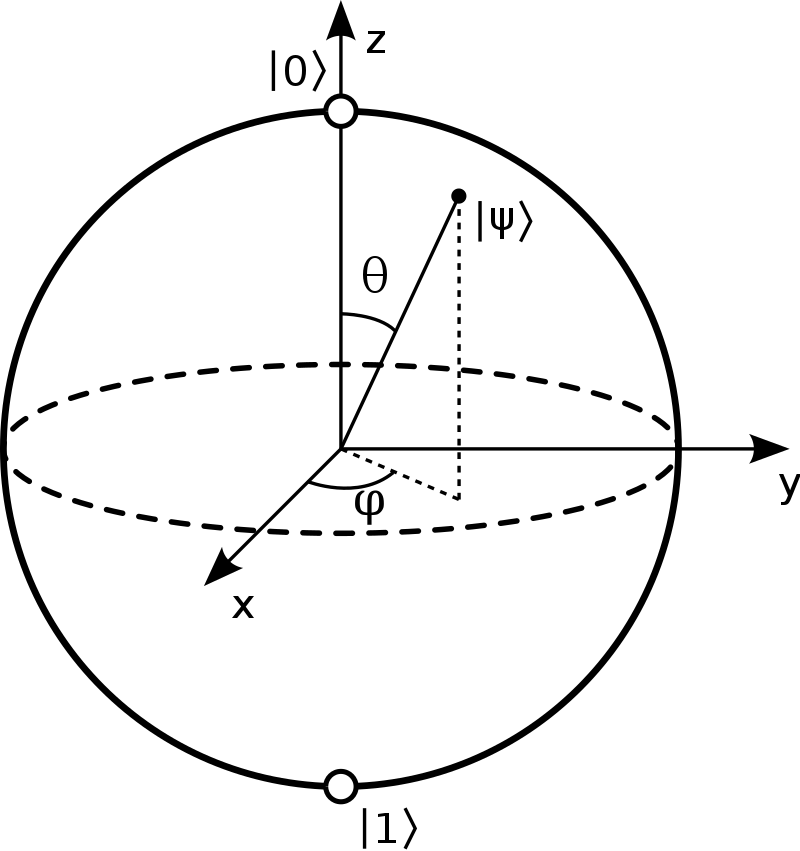
\includegraphics[width=0.45\columnwidth]{figs/Bloch_sphere.png}
    \label{fig:bloch_sphere}
    \caption{Sfera Blocha}
\end{figure}

Możemy połączyć oba przedstawienia tj. przedstawienia operatora i wektora stanu jeśli tylko zamiast
wektora stanu użyjemy operatora rzutowania na stan \(\Psi\). Możemy rozłożyć go wówczas (jak każdy
operator samosprzężony) na macierze Pauliego
\begin{equation*}
    \ket{\Psi}\bra{\Psi} = s_0\oper{I} + \mathbf{s}\cdot\boldsymbol{\sigma}\,,
\end{equation*}
przy czym parametry \(s_0,s_x,s_y,s_z\) muszą spełniać
\begin{equation*}
    \ket{\Psi}\bra{\Psi}\ket{\Psi}\bra{\Psi} = \ket{\Psi}\bra{\Psi}\,,
\end{equation*}
czyli
\begin{equation*}
    s_0\oper{I} + \mathbf{s}\cdot\boldsymbol{\sigma} = (s_0^2 + |\mathbf{s}|^2)\oper{I} + 2s_0\mathbf{s}\cdot\boldsymbol{\sigma}\,,
\end{equation*}
skąd \(s_0 = |\mathbf{s}| = 1/2\). Operator rzutowania \(\ket{\Psi}\bra{\Psi}\) możemy zatem w
ogólności rozłożyć na macierze Pauliego w następujący sposób
\begin{equation*}
    \ket{\Psi}\bra{\Psi} = \frac{1}{2}(\oper{I} + \mathbf{s}\cdot\boldsymbol{\sigma})\,,
\end{equation*}
gdzie przeskalowaliśmy zmienne \(s_x,s_y,s_z\) tak, że teraz \(\boxed{|\mathbf{s}| = 1}\).

Widzimy więc, iż stan \(\Psi\) możemy reprezentować jako wektor \(\mathbf{s}\) określający punkt na
sferze jednostkowej w trójwymiarowej przestrzeni, a operator samosprzężony jako dowolny wektor
\(\mathbf{a}\) w tej przestrzeni. Przejście od rzeczywistego wektora \(\mathbf{s}\) do
abstrakcyjnego wektora stanu \(\ket{\Psi}\) odbywa sie poprzez określenie współrzędnych sferycznych
\((\theta,\phi)\) wektora \(\mathbf{s}\) i zmapowanie ich zgodnie z przepisem
\begin{equation*}
    \ket{\Psi} = \cos\frac{\theta}{2}\ket{0} + \e^{\im\phi}\sin\frac{\theta}{2}\ket{1}\,.
\end{equation*}


\subsubsection{Ewolucja układu dwupoziomowego}

Dla układów dwupoziomowych ogólne równania ewolucji amplitud prawdopodobieństwa wektora stanu
\begin{equation*}
    \ket{\Psi} = \mqty[\alpha \\ \beta]
\end{equation*}
dla hamiltonianu postaci
\begin{equation*}
    \oper{H} = \mqty[H_{11}(t) & H_{12}(t) \\ H_{21}(t) & H_{22}(t)]
\end{equation*}
mają postać
\begin{equation*}\boxed{
    \begin{cases}
        \im\hbar\dot{\alpha} = H_{11}(t)\alpha + H_{12}(t)\beta\\
        \im\hbar\dot{\beta}  = H_{21}(t)\alpha + H_{22}(t)\beta
    \end{cases}}
\end{equation*}
Równanie ewolucji możemy zapisać również wykorzystując przedstawienie geometryczne wektorów stanu i
operatorów na sferze Blocha. Istotnie różniczkując operator rzutowy \(\oper{\rho} =
\ket{\Psi}\bra{\Psi}\) mamy
\begin{equation*}
    \begin{split}
        \pdv{\oper{\rho}}{t} &= \ket{\dot{\Psi}}\bra{\Psi} + \ket{\Psi}\bra{\dot{\Psi}} = \frac{1}{\im\hbar}\ket{\oper{H}\Psi}\bra{\Psi} - \frac{1}{\im\hbar}\ket{\Psi}\bra{\oper{H}\Psi}\\
        &=\frac{1}{\im\hbar}(\oper{H}\oper{\rho}-\oper{\rho}\oper{H}) = \frac{1}{\im\hbar}[\oper{H},\oper{\rho}]\,.
    \end{split}
\end{equation*}

Z powyższego mamy więc dla \(\oper{\rho} = \frac{1}{2}(\oper{I} +
\mathbf{s}\cdot\boldsymbol{\sigma})\) i \(\oper{H} = \mathbf{H}(t)\cdot\boldsymbol{\sigma}\)
\begin{equation*}\boxed{
    \frac{\hbar}{2}\dot{\mathbf{s}} = \mathbf{H}(t)\times\mathbf{s}}
\end{equation*}

Przedstawienie geometryczne wektora stanu na sferze Blocha nie jest jedynie obserwacją matematyczną.
Pozwala ono zwizualizować semi-klasyczną ewolucję wektorowej wielkości fizycznej \(\mathbf{S}\)
\footnote{W mechanice kwantowej wielkość \(\boldsymbol{\mu} \propto \mathbf{S}\) jest spinowym
momentem magnetycznym cząstki kwantowej.}, której składowe \(S_x\), \(S_y\), \(S_z\) są w
przestrzeni \(\mathscr{H}\) reprezentowane przez samosprzężone operatory Pauliego \(\oper{X}\),
\(\oper{Y}\), \(\oper{Z}\). Istotnie zgodnie z twierdzeniem Ehrenfesta
\begin{equation*}
    \dv{\expval{\mathbf{S}}}{t} = \frac{\im}{\hbar}\bra{\Psi}[\oper{H}, \boldsymbol{\sigma}]\ket{\Psi} = \frac{\im}{\hbar}\bra{\Psi}\left([\oper{H},\oper{X}],[\oper{H},\oper{Y}],[\oper{H},\oper{Z}]\right)\ket{\Psi}\,.
\end{equation*}
Jednocześnie dla \(\oper{H} = \mathbf{H}\cdot\boldsymbol{\sigma}\)
\begin{equation*}\boxed{
    \begin{split}
        &[\oper{H},\oper{X}] = -2\im H_y\oper{Z} + 2\im H_z \oper{Y}\\
        &[\oper{H},\oper{Y}] = -2\im H_z\oper{X} + 2\im H_x \oper{Z}\\
        &[\oper{H},\oper{Z}] = -2\im H_x\oper{Y} + 2\im H_y \oper{X}
    \end{split}}\quad,
\end{equation*}
skąd
\begin{equation*}
    \frac{\hbar}{2}\dv{\expval{\mathbf{S}}}{t} = \mathbf{H} \times \expval{\mathbf{S}}\,.
\end{equation*}
Widzimy zatem, iż ruch wektora \(\mathbf{s}\) po sferze Blocha odpowiada ewolucji wartości
oczekiwanej wielkości fizycznej \(\mathbf{S}\), którą to ewolucję możemy w przybliżeniu
semi-klasycznym traktować jako faktyczną ewolucję tych wielkości.

\subsubsection{Obroty na sferze Blocha}

Powyższe rozważania pokazują, iż w przedstawieniu geometrycznym stan \(\Psi\) reprezentowany przez
jednostkowy wektor \(\mathbf{s}\) na sferze Blocha ewoluuje w taki sposób, iż efektywnie jego
położenie na sferze Blocha w czasie \(t\) można przedstawić jako obrót wektora położenia w czasie
\(t_0\) o pewien kąt \(\varphi\) wokół ustalonej osi \(\mathbf{\hat{n}}\)
\begin{equation*}
    \mathbf{s}(t) = \overleftrightarrow{\mathbf{R}}_\mathbf{\hat{n}}(\varphi)\mathbf{s}(t_0)\,.
\end{equation*}
W ujęciu abstrakcyjnego wektora \(\ket{\Psi}\) przekształcenie to odpowiada oczywiście pewnemu
przekształceniu unitarnemu \(\oper{U}\), tj.
\begin{equation*}
    \ket{\Psi(t)} = \oper{U}\ket{\Psi(t_0)}\,.
\end{equation*}
Warte zbadania wydaje się więc wyznaczenie operatora \(\oper{U}\), który odpowiada obrotowi na
sferze Blocha. Aby wyznaczyć jawny wzór na operator \(\oper{U}\) rozważmy infinitezymalny obrót
wektora \(\mathbf{s}\) wokół osi \(\mathbf{\hat{n}}\) o kąt \(\epsilon\). Jak łatwo pokazać
\begin{equation*}
    \mathbf{s}' = \overleftrightarrow{\mathbf{R}}_\mathbf{\hat{n}}(\epsilon)\mathbf{s} = \mathbf{s} + \epsilon(\mathbf{s}\times\mathbf{\hat{n}})
\end{equation*}
w przybliżeniu do wyrazów liniowych względem \(\epsilon\). Wektor rzeczywisty \(\mathbf{s}\)
najłatwiej powiązać z abstrakcyjnym wektorem \(\ket{\Psi}\) poprzez operator rzutowy \(\oper{\rho} =
\ket{\Psi}\bra{\Psi}\) dla którego zachodzi
\begin{equation*}
    \ket{\oper{U}\Psi}\bra{\oper{U}\Psi} = \oper{U}\oper{\rho}\oper{U}^\dagger = \frac{1}{2}\left(\oper{I} + \mathbf{s}'\cdot\boldsymbol{\sigma}\right)\,,
\end{equation*}
skąd
\begin{equation*}
    \mathbf{s}\cdot\oper{U}\boldsymbol{\sigma}\oper{U}^\dagger = (\mathbf{s} + \epsilon(\mathbf{s}\times\mathbf{\hat{n}}))\cdot\boldsymbol{\sigma} = \mathbf{s}\cdot(\boldsymbol{\sigma} + \epsilon(\mathbf{\hat{n}}\times\boldsymbol{\sigma}))\,.
\end{equation*}
Otrzymujemy zatem równanie
\begin{equation*}
    \oper{U}\boldsymbol{\sigma}\oper{U}^\dagger = \boldsymbol{\sigma} + \epsilon(\mathbf{\hat{n}}\times\boldsymbol{\sigma})\,.
\end{equation*}
Poszukajmy \(\oper{U}\) spełniających to równanie postaci
\begin{equation*}
    \oper{U} = \oper{I} + \im\epsilon\oper{A}\,,\quad \oper{U}^\dagger = \oper{I} - \im\epsilon\oper{A}^\dagger\,,
\end{equation*}
gdzie \(\oper{A}\) jest operatorem samosprzężonym postaci \(\oper{A} =
\mathbf{a}\cdot\boldsymbol{\sigma}\). Zauważmy, iż tak zdefiniowany \(\oper{U}\) jest unitarny w
przybliżeniu do wyrazów liniowych względem \(\epsilon\). Podstawiając powyższe wzory na \(\oper{U}\)
oraz \(\oper{U}^\dagger\) i ograniczając się do wyrazów liniowych względem \(\epsilon\) otrzymujemy
\begin{equation*}
    \im\epsilon[\oper{A}, \boldsymbol{\sigma}] = \epsilon(\mathbf{\hat{n}}\times\boldsymbol{\sigma}).
\end{equation*}
Widzimy zatem, iż taki, a nie inny strzał na postać operatora \(\oper{U}\) był podyktowany
wyprowadzonymi wcześniej wzorami na komutatory operatora samosprzężonego z operatorami Pauliego,
które naśladują strukturę zwykłego trójwymiarowego iloczynu wektorowego. Z powyższego otrzymujemy
zatem \(\mathbf{a} = \frac{1}{2}\mathbf{\hat{n}}\), skąd
\begin{equation*}\boxed{
    \oper{U} = \oper{I} + \frac{\im \epsilon}{2} \mathbf{\hat{n}} \cdot \boldsymbol{\sigma}}\,.
\end{equation*}
Stąd łatwo możemy już uzyskać operator unitarny \(\oper{U}_\mathbf{\hat{n}}(\varphi)\) odpowiadający
obrotowi o kąt \(\varphi\) wokół osi \(\mathbf{\hat{n}}\)
\begin{equation*}\boxed{
    \oper{U}_\mathbf{\hat{n}}(\varphi) = \lim_{N\to\infty}\left(\oper{I} + \frac{\im \varphi}{2N} \mathbf{\hat{n}} \cdot \boldsymbol{\sigma}\right)^N = \exp{\frac{\im}{2}\varphi\mathbf{\hat{n}}\cdot\boldsymbol{\sigma}} = \oper{I}\cos\frac{\varphi}{2} + \im(\mathbf{\hat{n}}\cdot\boldsymbol{\sigma})\sin\frac{\varphi}{2}}
\end{equation*}
W szczególności dla obrotów wokół osi \(x\), \(y\), \(z\) mamy odpowiednio
\begin{equation*}\boxed{
    \begin{split}
        &\oper{U}_\mathbf{\hat{x}}(\varphi) = \mqty[\cos\frac{\varphi}{2} & \im\sin\frac{\varphi}{2} \\ \im\sin\frac{\varphi}{2} & \cos\frac{\varphi}{2}]\\
        &\oper{U}_\mathbf{\hat{y}}(\varphi) = \mqty[\cos\frac{\varphi}{2} & \sin\frac{\varphi}{2} \\ -\sin\frac{\varphi}{2} & \cos\frac{\varphi}{2}]\\
        &\oper{U}_\mathbf{\hat{z}}(\varphi) = \mqty[\e^{+\im\varphi/2} & 0 \\ 0 & \e^{-\im\varphi/2}]
    \end{split}}\quad.
\end{equation*}

\subsubsection{Przykłady}

\textbf{Magnetyczny rezonans jądrowy.} Rozważymy teraz zjawisko rezonansu magnetycznego mające
liczne zastosowania w wielu działach fizyki współczesnej. Rozpatrzmy cząstkę obdarzoną momentem
magnetycznym \(\mu\), lecz nie posiadającą ładunku elektrycznego (przypadek neutronu), która została
umieszczona w wirującym z częstością radiową polu magnetycznym
\begin{equation*}
    \mathbf{B}(t) = B_\text{rf}\cos(\omega t)\mathbf{\hat{x}} - B_\text{rf}\sin(\omega t) \mathbf{\hat{y}} + B_0\mathbf{\hat{z}}\,.
\end{equation*}
Hamiltonian interesującego nas układu dwupoziomowego ma postać
\begin{equation*}
    \oper{H} = -\mu\mathbf{B}\cdot\boldsymbol{\sigma} = -\mu\mqty[B_0 & B_\text{rf}\e^{+\im\omega t} \\ B_\text{rf}\e^{-\im\omega t} & -B_0]\,.
\end{equation*}
Równania ewolucji na amplitudy prawdopodobieństwa mają więc postać
\begin{equation*}
    \begin{split}
        &\frac{1}{\im\omega_0}\dot{\alpha} =\eta\e^{+\im\omega t}\beta + \alpha \\
        &\frac{1}{\im\omega_0}\dot{\beta} = \eta\e^{-\im\omega t}\alpha - \beta
    \end{split}\quad,
\end{equation*}
gdzie wprowadziliśmy parametry \(\omega_0 := \mu B_0 / \hbar\) i \(\eta := B_\text{rf}/B_0\).
Poszukajmy rozwiązań postaci
\begin{equation*}
    \mqty[\alpha\\\beta] = \mqty[\phi_1(t)\e^{+\im\omega t/2} \\ \phi_2(t)\e^{-\im\omega t/2}]\,.
\end{equation*}
Po podstawieniu otrzymujemy układ równań
\begin{equation*}
    \frac{1}{\im\omega_0}\mqty[\dot{\phi}_1 \\ \dot{\phi}_2] = \mqty[\xi & \eta \\ \eta & -\xi]\mqty[\phi_1 \\ \phi_2]\,,
\end{equation*}
gdzie \(\xi = 1 - \frac{\omega}{2\omega_0}\). Powyższy układ równań możemy łatwo rozwiązać
poszukując rozwiązań postaci
\begin{equation*}
    \mqty[\phi_1(t) \\ \phi_2(t)] = \mqty[\Phi_1 \\ \Phi_2] \e^{\im\omega_0\lambda t}\,,
\end{equation*}
co po podstawieniu prowadzi do zagadnienia własnego
\begin{equation*}
    \mqty[\xi & \eta \\ \eta & -\xi]\mqty[\Phi_1 \\ \Phi_2] = \lambda \mqty[\Phi_1 \\ \Phi_2]\,.
\end{equation*}
Łatwo sprawdzić, iż wartości i wektory własne wynoszą odpowiednio
\begin{equation*}
    \lambda_\pm = \pm \sqrt{\xi^2 + \eta^2}\,,\quad \mqty[\Phi_1 \\ \Phi_2] = a_\pm\mqty[\frac{\eta}{\lambda_\pm - \xi} \\ 1]\,.
\end{equation*}
Rozwiązanie ma zatem postać
\begin{equation*}
    \mqty[\phi_1 \\ \phi_2] = a_+\mqty[\frac{\eta}{\lambda_+-\xi}\\1]\e^{+\im\Omega t} + a_-\mqty[\frac{\eta}{\lambda_--\xi}\\1]\e^{-\im\Omega t}\,,
\end{equation*}
gdzie \(\boxed{\Omega := \sqrt{\left(\omega_0 - \frac{1}{2}\omega\right)^2 +
\left(\frac{\omega_0B_\text{rf}}{B_0}\right)^2}}\) to tzw. \textit{częstość Rabiego}. Załóżmy, iż w
chwili początkowej \(\alpha = 0\) i \(\beta = 1\), wówczas
\begin{equation*}
    a_+ = \frac{\lambda_+ - \xi}{\lambda_+ - \lambda_-}\,,\quad a_- = 1 - a_+ = \frac{-\lambda_-+\xi}{\lambda_+ - \lambda_-}\,,
\end{equation*}
skąd
\begin{equation*}
    \begin{split}
        &\alpha(t) = \frac{\im\omega_0B_\text{rf}}{\Omega B_0}\sin(\Omega t)\e^{+\im\omega t/2}\\
        &\beta(t) = \left\{\cos(\Omega t) +\frac{\im}{\Omega}\left(\frac{1}{2}\omega - \omega_0\right)\sin(\Omega t)\right\}\e^{-\im\omega t/2}
    \end{split}\quad.
\end{equation*}
Z powyższego prawdopodobieństwo \(p_{1\to0}\) znalezienia układu w stanie \(\ket{0}\) wynosi
\begin{equation*}
        p_{1\to0}(t) = |\alpha|^2 = \left(\frac{\omega_0B_\text{rf}}{\Omega B_0}\right)^2\sin^2(\Omega t) = \frac{1}{2}\left(\frac{\omega_0B_\text{rf}}{\Omega B_0}\right)^2(1-\cos(2\Omega t))\,.
\end{equation*}
Natomiast prawdopodobieństwo \(p_{1\to1}\) znalezienia układu w stanie \(\ket{1}\) wynosi
\begin{equation*}
        p_{1\to1}(t) = |\beta|^2 =\cos^2(\Omega t) + \left(\frac{\omega_0 - \frac{1}{2}\omega}{\Omega}\right)^2\sin^2(\Omega t) = 1 - p_{1\to 0}(t)\,.
\end{equation*}
Prawdopodobieństwa oscylują w czasie z częstością równą podwojonej częstości Rabiego. Amplituda tych
oscylacji wynosi
\begin{equation*}
    \frac{1}{2}\left(\frac{\omega_0B_\text{rf}}{\Omega B_0}\right)^2 = \frac{\omega_0^2B_\text{rf}^2}{2B_0^2}\frac{1}{\left(\omega_0 - \frac{1}{2}\omega\right)^2 +
    \left(\frac{\omega_0B_\text{rf}}{B_0}\right)^2}
\end{equation*}
i przyjmuje wartość maksymalną, gdy spełniony jest \textit{warunek rezonansu} postaci
\begin{equation*}
    \boxed{\hbar\omega = 2\mu B_0}
\end{equation*}
\begin{figure}[ht]
    \centering
    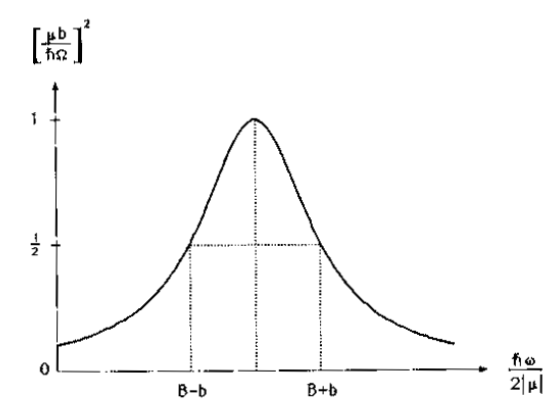
\includegraphics[width=0.7\columnwidth]{figs/nmr.png}
    \caption{Wykres podwojonej amplitudy oscylacji Rabiego w funkcji częstości pola magnetycznego.
    Na powyższym wykresie \(b=B_\text{rf}\) i \(B=B_0\)}
\end{figure}

Zauważmy, iż opisane zjawisko stanowi podstawę do manipulacji qbitami. Istotnie w stanie rezonansu
wektor stanu ewoluuje zgodnie z
\begin{equation*}
    \ket{\Psi(t)} = \alpha(t)\ket{0} + \beta(t)\ket{1} = \im\sin(\Omega t)\e^{+\im\omega_0 t}\ket{0} + \cos(\Omega t)\e^{-\im\omega_0 t}\ket{1}
\end{equation*}
Poprzez dostosowanie czasu \(t\) przez jaki układ dwupoziomowy oddziałuje z wirowym polem możemy
sterować stanem \(\Psi\) w jakim się znajduje, przykładowo jeśli początkowo układ był w stanie
\(\ket{1}\) to włączając wirowe pole magnetyczne na czas \(t = \pi/2\Omega\) układ przechodzi do
stanu \(\ket{0}\) (pomijając nieistotny globalny czynnik fazowy).

\linesep

\textbf{Precesja momentu magnetycznego.} Rozważmy ponownie cząstkę obdarzoną momentem magnetycznym,
ale nie obdarzoną ładunkiem elektrycznym, która została umieszczona w jednorodnym polu magnetycznym
\(\mathbf{B} = B(t)\mathbf{\hat{z}}\). Równania ewolucji składowych wektora na sferze Blocha mają
postać
\begin{equation*}
    \frac{\hbar}{2}\dot{s}_x = +\mu B s_y\,,\quad \frac{\hbar}{2}\dot{s}_y = -\mu Bs_x\,,\quad \frac{\hbar}{2}\dot{s}_z = 0
\end{equation*}
skąd \(s_z = \text{const.}\) natomiast sprzężone równania na \(s_x\) i \(s_y\) możemy rozdzielić
wprowadzając zmienne zespolone
\begin{equation*}
    \xi = s_x + \im s_y\,,\quad \eta = s_x - \im s_y = \xi^*\,,
\end{equation*}
dla których zachodzi
\begin{equation*}
    \begin{split}
        &\frac{\hbar}{2}\dot{\xi} = \mu B s_y - \im \mu B s_x = -\im \mu B \xi\\
        &\frac{\hbar}{2}\dot{\eta} = \mu B s_y + \im \mu B s_x = +\im \mu B \eta
    \end{split}\quad,
\end{equation*}
skąd
\begin{equation*}
    \begin{split}
        \xi(t) = a\exp(-\frac{2\im\mu}{\hbar}\int\limits_0^tB(t')\dd{t'} - \im\delta)\\
        \eta(t) = a\exp(+\frac{2\im\mu}{\hbar}\int\limits_0^tB(t')\dd{t'} + \im\delta)
    \end{split}\quad,
\end{equation*}
Z powyższego mamy więc
\begin{equation*}
    \begin{split}
        &s_x = \frac{\xi + \eta}{2} = a \cos(\frac{2\mu}{\hbar}\int\limits_0^tB(t')\dd{t'} + \delta)\\
        &s_y = \frac{\xi - \eta}{2\im} = -a\sin(\frac{2\mu}{\hbar}\int\limits_0^tB(t')\dd{t'} + \delta)\\
        &s_z = \text{const.}
    \end{split}\quad.
\end{equation*}
Równania te opisują precesję wektora \(\mathbf{s}\) wokół osi \(z\) z zależną od czasu częstością. W
szczególnym przypadku \(B(t) = B_0\) mamy
\begin{equation*}
    s_x = a\cos(\omega_\text{L}t + \delta)\,,\quad s_y = -a\sin(\omega_\text{L}t + \delta)\,,\quad s_z=\text{const.}\,,
\end{equation*}
gdzie \(\boxed{\omega_\text{L} = 2\mu B_0/\hbar }\) to tzw. \textit{częstość Larmora}.

\subsection{Twierdzenie adiabatyczne}

\begin{theorem}[\textit{adiabatyczne}]
    Niech \(\oper{H}(t)\) będzie hamiltonianem (o dyskretnym i niezdegenerowanym spektrum) pewnego
    układu kwantowego, który zmienia się \textit{bardzo powoli} (adiabatycznie) \(\oper{H}(t_i) \to
    \oper{H}(t_f)\) w czasie \(\Delta t = t_f - t_i\). Wówczas jeśli układ w chwili początkowej
    \(t_i\) znajdował się w \(n\)--tym stanie własnym hamiltonianu \(\oper{H}(t_i)\) to po
    adiabatycznej ewolucji w chwili końcowej \(t_f\) będzie znajdował się w \(n\)--tym stanie
    własnym hamiltonianu \(\oper{H}(t_f)\).
\end{theorem}

Niech \(\{\psi_n(t)\}\) będzie zbiorem wektorów własnych hamiltonianu \(\oper{H}(t)\). Funkcję
falową \(\Psi\) w chwili \(t\) możemy zatem zapisać jako
\begin{equation*}
    \ket{\Psi(t)} = \sum_n c_n(t)\ket{\psi_n(t)}
\end{equation*}
gdzie \(\oper{H}(t)\ket{\psi_n(t)} = \lambda_n(t)\ket{\psi_n(t)}\). Jednocześnie z równania
Schr\"{o}dingera mamy
\begin{equation*}
    \begin{split}
        \oper{H}(t)\ket{\Psi(t)} &= \sum_n c_n(t) \lambda_n(t)\ket{\psi_n(t)} = \im\hbar\partial_t\ket{\Psi(t)} \\
        &= \im\hbar \sum_n \left(\dot{c}_n(t)\ket{\psi_n(t)} + c_n(t)\ket{\dot{\psi}_n(t)}\right)
    \end{split}
\end{equation*}
Działając na powyższe równanie \(\bra{\psi_m(t)}\) otrzymujemy
\begin{equation*}
    \lambda_m(t)c_m(t) = \im\hbar\dot{c}_m(t) + \im\hbar\sum_n c_n(t) \braket{\psi_m(t)}{\dot{\psi}_n(t)}\,.
\end{equation*}
Różniczkując równanie własne mamy natomiast
\begin{equation*}
    \dot{\oper{H}}(t)\ket{\psi_n(t)} + \oper{H}(t)\ket{\dot{\psi}_n(t)} = \dot{\lambda}_n(t)\ket{\psi_n(t)} + \lambda_n(t)\ket{\dot{\psi}_n(t)}\,.
\end{equation*}
Działając na to równanie \(\bra{\psi_m(t)}\) oraz pamiętając, iż z tw. spektralnego 
\begin{equation*}
    \oper{H}(t) = \sum_n \lambda_n(t) \ket{\psi_n(t)}\bra{\psi_n(t)}
\end{equation*}
otrzymujemy
\begin{equation*}
    \begin{split}
        &\bra{\psi_m(t)}\dot{\oper{H}}(t)\ket{\psi_n(t)} + \lambda_m(t)\braket{\psi_m(t)}{\dot{\psi}_n(t)} \\
        &= \dot{\lambda}_n(t)\braket{\psi_m(t)}{\psi_n(t)} + \lambda_n(t)\braket{\psi_m(t)}{\dot{\psi}_n(t)}
    \end{split}\quad.
\end{equation*}
Dla \(m \neq n\) mamy więc
\begin{equation*}
    \braket{\psi_m(t)}{\dot{\psi}_n(t)} = \frac{\bra{\psi_m(t)}\dot{\oper{H}}(t)\ket{\psi_n(t)}}{\lambda_n(t) - \lambda_m(t)}\,.
\end{equation*}
Możemy zatem zapisać równanie ewolucji na współczynniki \(c_m\) jako
\begin{equation*}
    -\dot{c}_m(t) = \left[\frac{\im}{\hbar}\lambda_m(t) + \braket{\psi_m(t)}{\dot{\psi}_m(t)}\right]c_m(t) + \sum_{n \neq m} c_n(t) \frac{\bra{\psi_m(t)}\dot{\oper{H}}(t)\ket{\psi_n(t)}}{\lambda_n(t) - \lambda_m(t)}
\end{equation*}
Przybliżenie adiabatyczne polega na pominięciu drugiego członu po prawej stronie tj. zakładamy że w
każdej chwili \(t\) widmo hamiltonianu jest niezdegenerowane czyli \(\forall t: \forall n\neq m:
\lambda_n(t) \neq \lambda_m(t)\) oraz zakładamy, iż pochodna hamiltonianu jest bardzo mała. Wówczas mamy
\begin{equation*}\boxed{
    \dot{c}_m(t) \approx \im \left[-\frac{1}{\hbar}\lambda_m(t) + \im\braket{\psi_m(t)}{\dot{\psi}_m(t)}\right] c_m(t)}
\end{equation*}
skąd rozwiązanie to
\begin{equation*}
    c_m(t) = c_m(0)\e^{\im\theta_m(t)}\e^{\im\gamma_m(t)}\,,
\end{equation*}
gdzie
\begin{equation*}
    \theta_m(t) := -\frac{1}{\hbar}\int\limits_0^t \lambda_m(t')\dd{t'} \in \mathbb{R}
\end{equation*}
to tzw. \textit{faza dynamiczna}, a
\begin{equation*}
    \gamma_m(t) := \im\int\limits_0^t \braket{\psi_m(t')}{\dot{\psi}_m(t')} \dd{t'} \in \mathbb{R}
\end{equation*}
to tzw. \textit{faza geometryczna}. Aby przekonać się, iż \(\gamma_m \in \mathbb{R}\) wystarczy zróżniczkować warunek unormowania 
\begin{equation*}
    0 = \dv{\braket{\psi_m}}{t} = \braket{\psi_m}{\dot{\psi}_m}^* + \braket{\psi_m}{\dot{\psi}_m} = 2\Re{\braket{\psi_m}{\dot{\psi}_m}}\,.
\end{equation*}


\newpage
\section{Obliczenia kwantowe}









\end{document}
